\section{MorphoLab: công cụ hỗ trợ thực nghiệm}
Ứng dụng desktop được xây dựng để giảm thao tác khi đổi tham số, xem ảnh trung gian và chạy kiểm chứng. Phần lõi vẫn là các hàm Python đã trình bày; kết quả gọi từ giao diện và CLI có cùng quy ước dữ liệu. Ứng dụng là sản phẩm bổ trợ cho nghiên cứu, không phải tiêu chí thay thế nội dung thuật toán, thực nghiệm hoặc đánh giá định lượng.

Sáu tab gồm Phân đoạn, Fiji \& đánh giá, Benchmark, Nghiên cứu, Phiên đã lưu và Hướng dẫn. Giao diện giải thích thuật ngữ tiếng Anh bằng tiếng Việt: marker (hạt giống), mask (miền tiền cảnh), ground truth (nhãn đúng), split/merge (chia thừa/gộp sai). Cảnh báo kết quả cũ giúp tránh thay tham số rồi vô tình xuất kết quả của lần chạy trước.

\begin{figure}[htbp]\centering
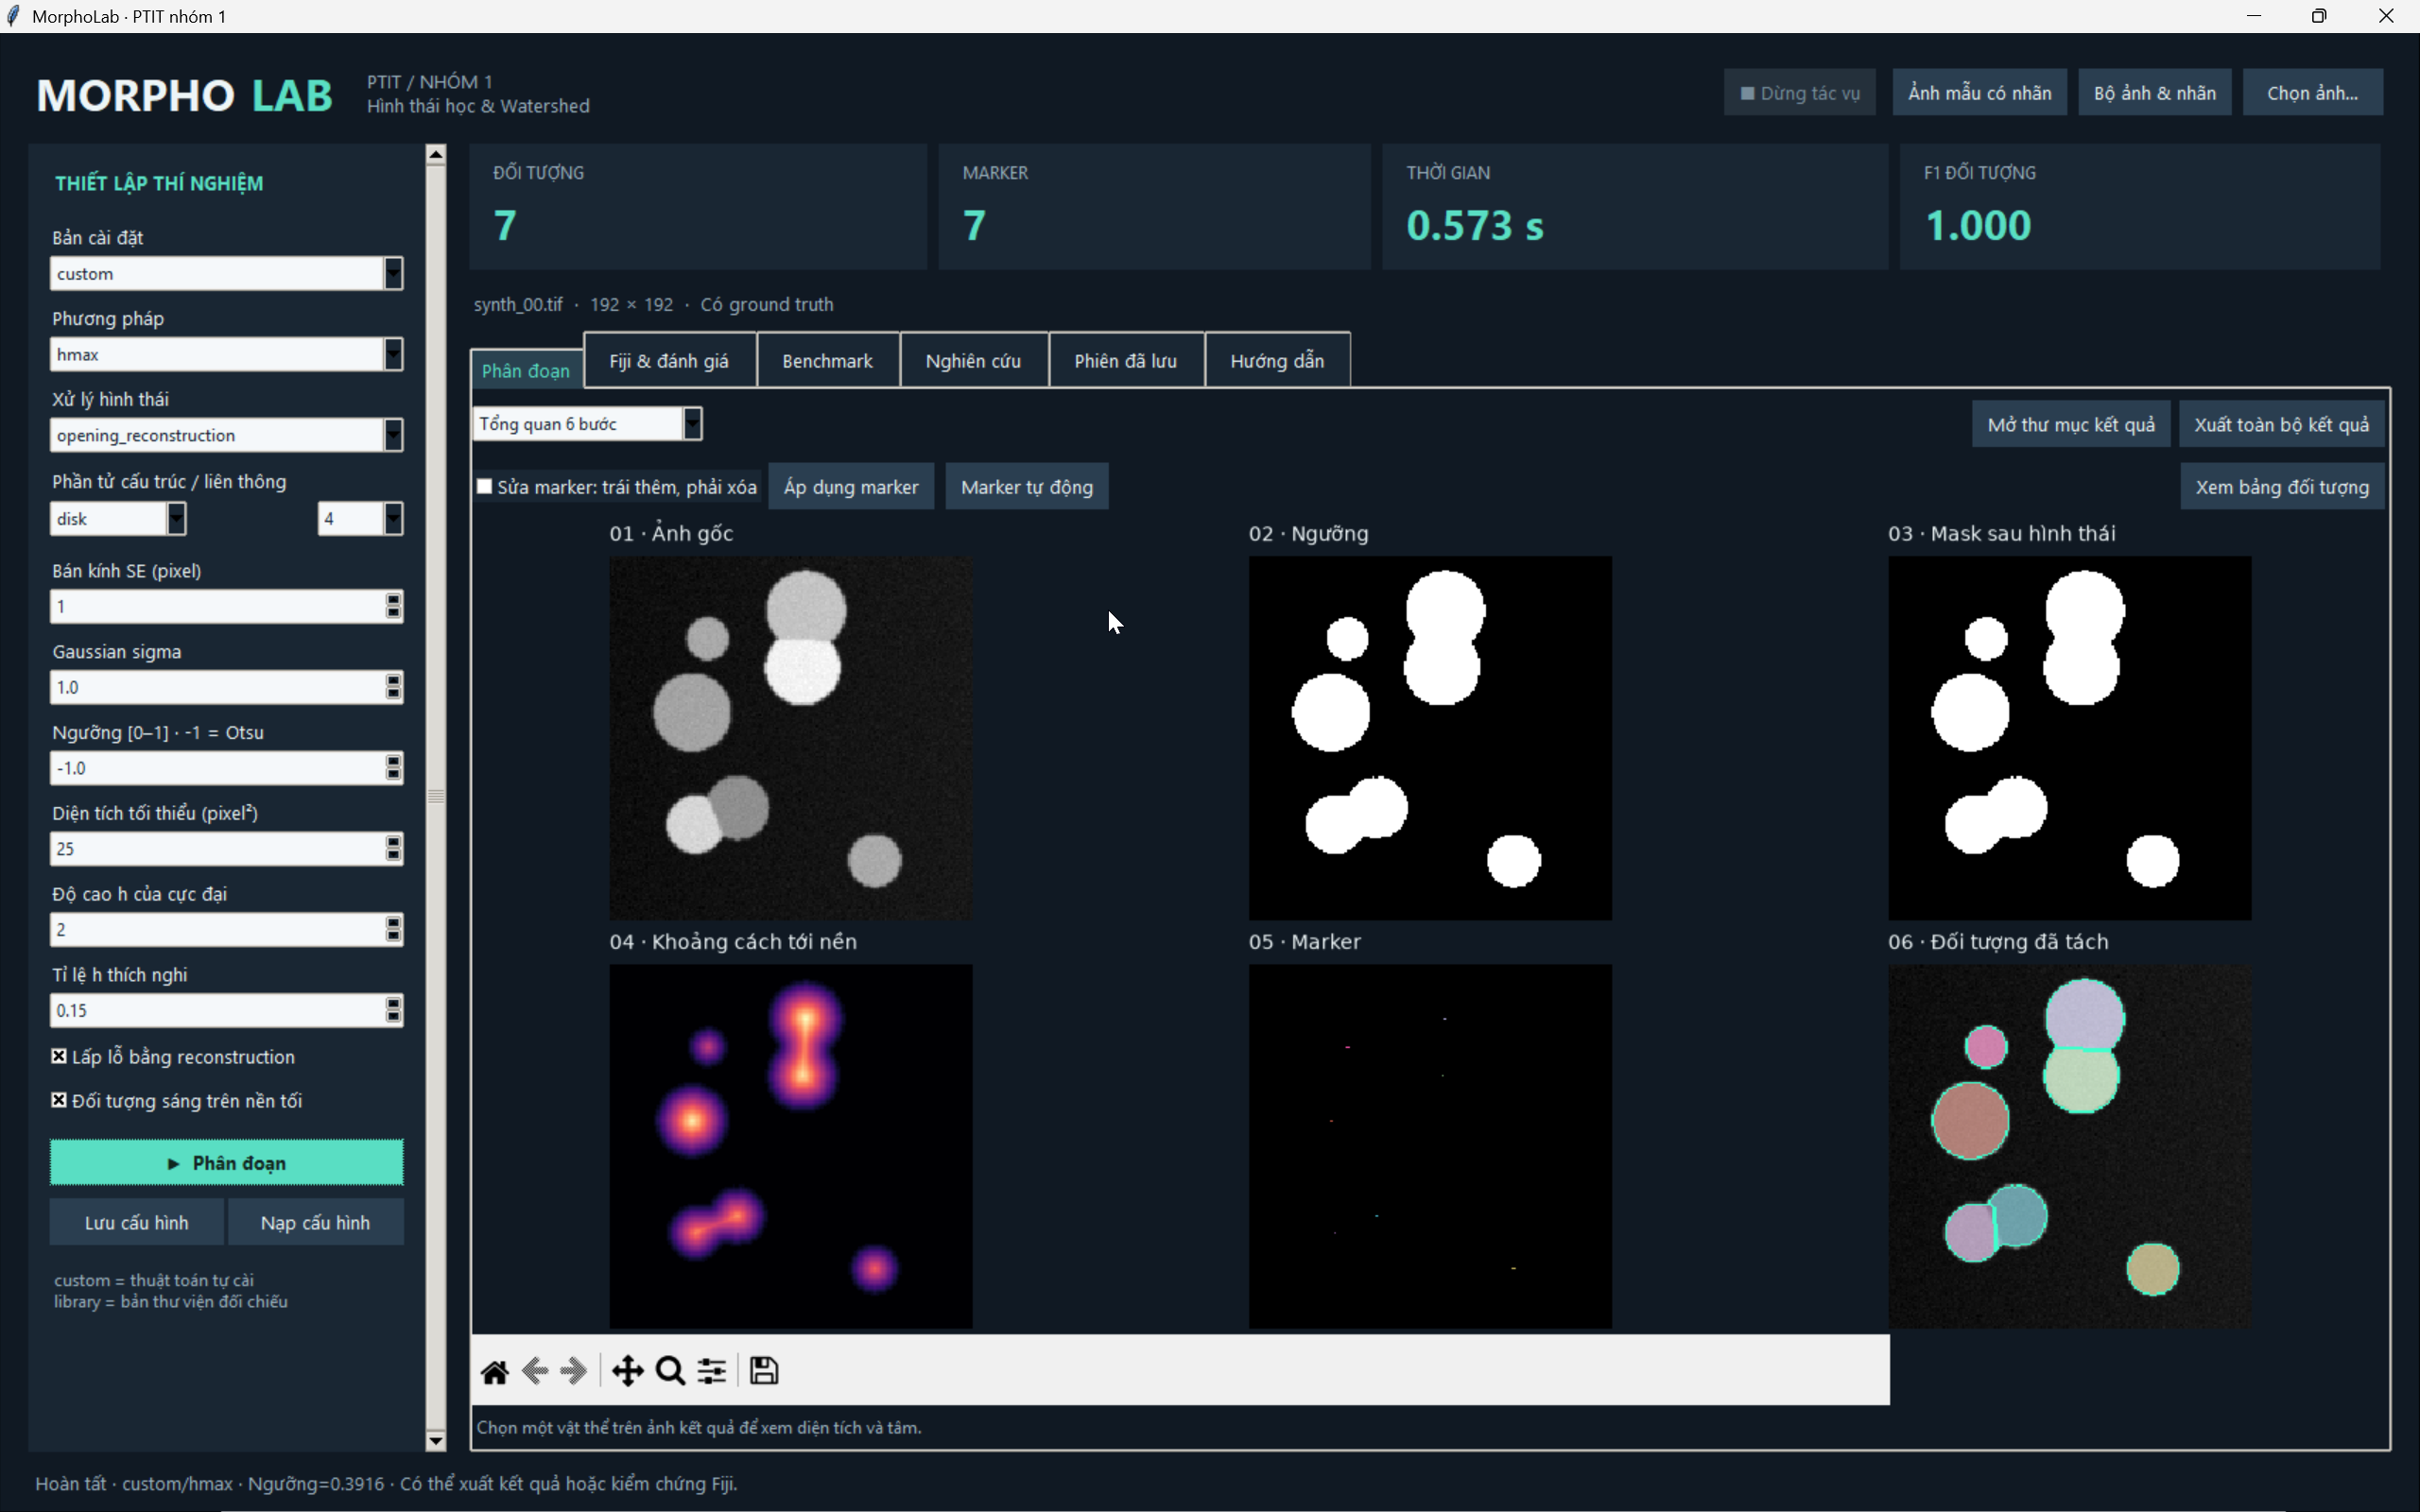
\includegraphics[width=\linewidth]{figures/morpholab_app.png}
\caption{MorphoLab hiển thị sáu bước trên ảnh mẫu: 7 đối tượng, 7 marker, F1 = 1. Ảnh chụp ứng dụng do người học cung cấp trong quá trình thực hành; thời gian hiển thị thuộc lần chạy đó.}\label{fig:app}
\end{figure}

\begin{table}[htbp]\centering\small
\caption{Chức năng ứng dụng gắn với công việc nghiên cứu.}\label{tab:app}
\begin{tabularx}{\linewidth}{X X}\toprule
Chức năng & Giá trị hỗ trợ \\\midrule
Xem sáu bước và từng ảnh trung gian & Giải thích nguyên nhân lỗi từ ngưỡng, mask hoặc marker.\\
Chỉnh marker bằng chuột & Thử giả thuyết về số hạt giống; kết quả thủ công được phân biệt với tự động.\\
Gọi Fiji shared/native & Kiểm chứng JAR thật và xem khác biệt; giữ hai giao thức rõ ràng.\\
Benchmark và kế hoạch nghiên cứu & Chạy nhiều ảnh tuần tự, xuất CSV/JSON/biểu đồ.\\
Lưu/mở phiên & Giữ ảnh, nhãn đúng, cấu hình và đầu ra để xem lại.\\
Xuất bảng đối tượng & Đọc diện tích, tâm và thuộc tính từng nhãn.\\\bottomrule
\end{tabularx}\end{table}

\section{Kịch bản dùng app để minh họa}
Mở \texttt{launch\_app.cmd} hoặc chạy \texttt{python -m morpholab gui} trong env \texttt{ai}. Chọn \textbf{Ảnh mẫu có nhãn}, giữ cấu hình mặc định và bấm \textbf{Phân đoạn ảnh}. Xem lần lượt ảnh gốc, phân ngưỡng, mask, distance, marker và nhãn. Đổi mode sang CCL để thấy năm vùng, rồi trở lại hmax để thấy bảy đối tượng. Mọi thay đổi phải bấm chạy lại trước khi so sánh hoặc xuất.

Sang \textbf{Fiji \& đánh giá}, chạy tham chiếu, xem nhãn Python/Fiji và vùng bất đồng. Nếu sửa marker, cần áp dụng marker trước; không trộn kết quả tương tác với kết quả tự động khi báo cáo F1. Các tab Benchmark/Nghiên cứu dùng cấu hình và dataset đã chọn; bắt đầu một ảnh trước khi chạy cả tập.

\section{Giới hạn của công cụ hỗ trợ}
Giao diện không làm thuật toán tự hiểu ngữ nghĩa ảnh. Thao tác người dùng có thể thay kết quả mạnh nên cấu hình, nhãn đầu vào và lịch sử chạy phải được giữ. Test phần mềm kiểm tra luồng thao tác và xuất dữ liệu, còn chất lượng phân đoạn vẫn phải đo với ground truth. Trong buổi bảo vệ, có thể demo bằng app nhưng phải chỉ được hàm xử lý và lệnh CLI tương ứng để tái lập độc lập.
